\documentclass[a4paper,12pt]{article} % добавить leqno в [] для нумерации слева

%%% Работа с русским языком
\usepackage{cmap}					% поиск в PDF
\usepackage{mathtext} 				% русские буквы в фомулах
\usepackage[T2A]{fontenc}			% кодировка
\usepackage[utf8]{inputenc}			% кодировка исходного текста
\usepackage[english,russian]{babel}	% локализация и переносы
\usepackage{float}
\usepackage{graphicx}
%%% Дополнительная работа с математикой
\usepackage{amsmath,amsfonts,amssymb,amsthm,mathtools} % AMS
\usepackage{icomma} % "Умная" запятая: $0,2$ --- число, $0, 2$ --- перечисление

%% Номера формул
%\mathtoolsset{showonlyrefs=true} % Показывать номера только у тех формул, на которые есть \eqref{} в тексте.

%% Шрифты
\usepackage{euscript}	 % Шрифт Евклид
\usepackage{mathrsfs} % Красивый матшрифт
\newtheorem{theorem}{Theorem}
\newtheorem{lemma}[theorem]{Lemma}
\theoremstyle{definition}
\newtheorem{definition}{Definition}[section]
%% Свои команды
\DeclareMathOperator{\sgn}{\mathop{sgn}}

%% Перенос знаков в формулах (по Львовскому)
\newcommand*{\hm}[1]{#1\nobreak\discretionary{}
	{\hbox{$\mathsurround=0pt #1$}}{}}

%%% Заголовок
\author{Илья Михеев}
\title{Интерферометр Майкльсона}
\date{last upd \today  }

\begin{document} % конец преамбулы, начало документа
	
	\maketitle 
	\section{Параметры установки}
	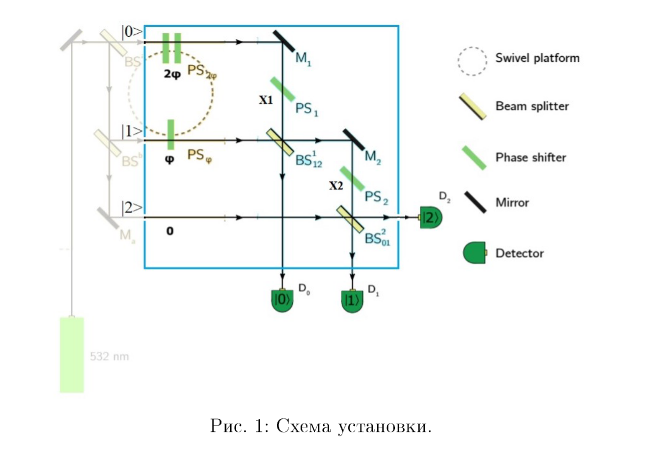
\includegraphics{Mint.png}
	Матрицы BS и PS можно записать как 
	\begin{equation*}
		P_n = \begin{bmatrix}
			e^{i(2\phi + x_n)}&0  & 0\\ 
			0& e^{i \phi} & 0\\ 
			0& 0 & 0
		\end{bmatrix}
	BS^1_{12} = \frac{1}{\sqrt{2}}\begin{bmatrix}
		1&i  & 0\\ 
		i&  1& 0\\ 
		0& 0 & \sqrt{2}
	\end{bmatrix}
	BS^2_{01} = \frac{1}{\sqrt{2}} \begin{bmatrix}
		\sqrt{2}&0  &0 \\ 
		0& 1 &i \\ 
		0& i & 1
	\end{bmatrix}
	\end{equation*}
	Тогда выходное состояние будет выглядеть как
	\begin{equation*}
		\psi_{out} = \begin{bmatrix}
		\frac{e^{i \phi}(i + e^{i(x_1 + \phi)})}{\sqrt{6}}&\frac{i \sqrt{2} + e^{i(x_2 + \phi) + i e^{i(x_2+x_1+2\phi)}}}{2 \sqrt{3}}&\frac{i \sqrt{2} + e^{i(x_2 + \phi) - i e^{i(x_2+x_1+2\phi)}}}{2 \sqrt{3}} \\ 
		\end{bmatrix}
	\end{equation*}
	Тогда 
	\begin{equation*}
		I^0(\phi, x_1) = \frac{1}{3} (1 + \sin(\phi + x_1))
	\end{equation*}
	\begin{equation*}
		I^1(\phi, x_1, x_2) = \frac{1}{6} (2 + \sqrt{2} \cos(\phi + x_1 + x_2) - \sin(x_1 + \phi) + \sqrt{2}\sin(x_2 + \phi))
	\end{equation*}
	Далее посчитаем $\alpha_0$ с помощью инетенсивности на нулевом детекторе. Если $\phi = 2\pi \frac{\alpha}{\alpha_0}$, то расстояние между 2 соседними минимумами --- $\alpha_0$. Исходя из графика, получаем, что $\alpha_0 \approx 0,003$.\\
	Посчитаем следующие интегралы:
	\begin{equation*}
		\int\limits_0^{2\pi} I^0(\phi, x_1) \sin (\phi) d\phi = \frac{1}{3} \pi \cos x_1
	\end{equation*}
	\begin{equation*}
		\int\limits_0^{2\pi} I^1(\phi, x_1, x_2) \cos (2\phi) d\phi = \frac{\pi \cos(x_1 + x_2)}{3 \sqrt{2}}
	\end{equation*}
	 С помощью этого определяем сдвиг фаз $x_1$ и $x_2$:
	 \begin{figure}[H]
	 	
	 	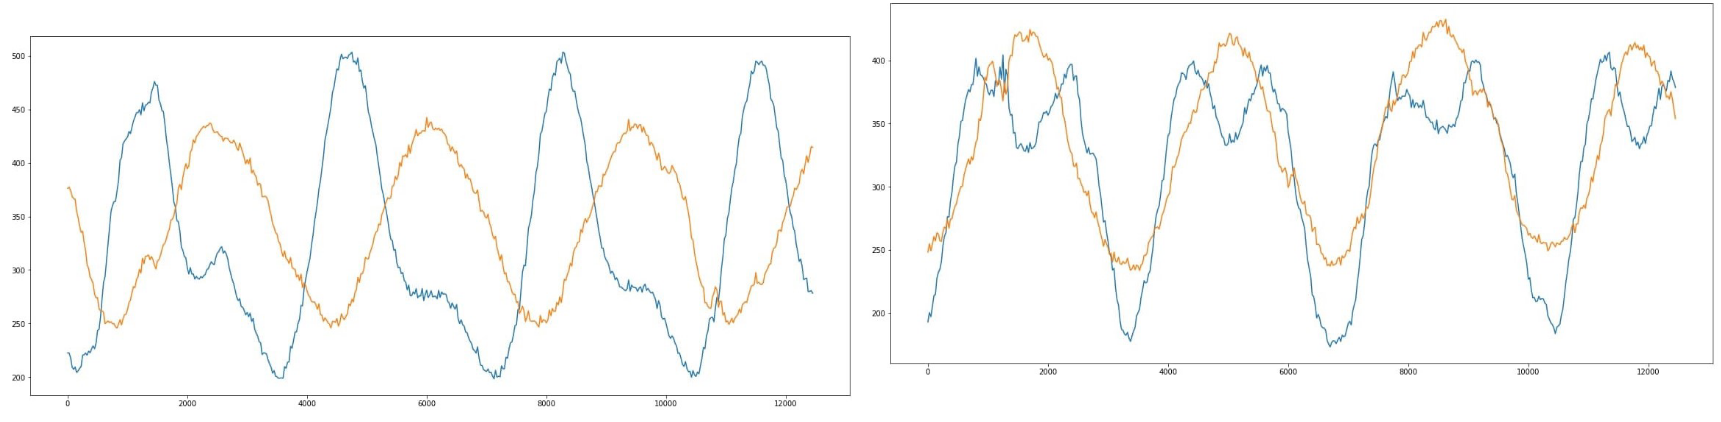
\includegraphics[width=\textwidth]{graph.png}
	 \end{figure}
	$x_1 = \arccos(0,04)$, $x_2 + x_1 = \arccos(-0,25)$.
\end{document} % конец документа
